\documentclass[modern]{aastex62}
\usepackage{hyperref}
% lsstdoc documentation: https://lsst-texmf.lsst.io/lsstdoc.html
\input{meta}

% Package imports go here.

% Local commands go here.



\newcommand{\docRef}{PSTN-052}
\newcommand{\docUpstreamLocation}{\url{https://github.com/lsst-pst/pstn-052}}


\begin{document}
\input{authors}
\date{\today}
\title{Survey Strategy: Rolling Cadence}
\hypersetup{pdftitle={\@title}, pdfauthor={\@author}, pdfkeywords={\@keywords}}

\begin{abstract}
We cover the basics of how a rolling cadence survey strategy can work, and review the results of a variety of rolling simulations. We find that Type Ia SNe recovery can be enhanced by using rolling cadence, while detecting fast microlensing events are dominated by footprint coverage.
\end{abstract}

\section{Introduction}

The Rubin Science Requirements Document \citep[SRD;][]{LPM-17} stipulated that Rubin should survey 18,000 square degrees with a median of 825 visits (spread over the $ugrizy$\ filters) after 10 years. This works out to one observation every 4.4 days (or one observation every 2.6 days if we have a 7-month observing season). For many transient phenomenon, including SNe Ia, this cadence is not ideal and something slightly higher (e.g., one observation every 2 days) would be preferred.

There is no free lunch. Once we have defined a survey footprint and telescope efficiency, the mean observing cadence is highly constrained. The additional preference to take observations near the meridian further constrains the possible cadence and season length. Going to higher cadence at one time demands that there be a corresponding period of lower cadence to ensure footprint coverage uniformity. Similarly, if an area has a higher cadence, another point at similar RA must also have a lower cadence because the telescope efficiency is fixed.  In Figure~\ref{fig:ideal_foot} we show the ideal cumulative number of observations for different observing strategies. Figure~\ref{fig:ideal_foot} also shows that {\bf{rolling and non-rolling cadences have the same mean and median cadence}}. When comparing simulations, it is important not to make approximations that average an observing cadence, as the effects of rolling will be lost.

The SRD also places tight constraints on the uncertainty in stellar proper motions. Proper motion uncertainties are dominated by the quality of astrometric measurements at the start and end of the survey. Thus, for all our rolling cadence simulations we use uniform coverage in the first and final 1.5 years of the survey. If we start rolling before 1.5 years, some areas of the sky will not have had a full observing season completed, thus they will have lower final proper motion precision than the areas of the sky that were covered for a full season.


\begin{figure}
\plotone{plots/footprint_ideal.pdf}
\caption{A comparison of how the cumulative number of observations varies at 4 points in the sky for non-rolling and rolling cadences. Note how when one point on the sky has higher cadence, a point at the same RA but different dec has lower cadence. Also, points at different RA's have different phases. \label{fig:ideal_foot}}
\end{figure}

\begin{figure}
\plotone{plots/actual_footprint.pdf}
\caption{A plot of the actual cumulative number of visits (all filters) for the point RA,dec = (0, -20). Right panel is a zoom in of the left. \label{fig:actual_foot}}
\end{figure}




Another constraint on the survey strategy is ensuring we have adequate images to construct image difference templates. We therefore usually do not simulate a ``full rolling" strategy where regions of the sky go completely unobserved for an entire season. The strength of the rolling is a free parameter, and we typically try to demand 3 observations per filter per year. In many simulations, we get slightly more than 15 observations per year. This can be caused by the scheduler not being able to focus on the rolling area of the sky, for example if the moon is in the way, forcing observations onto non-rolling areas.

Yet another potential limitation is the nature of the Rubin alert stream. If we construct the rolling cadence such that we concentrate observations on the southern sky for a year, that will mean the alert stream will be concentrated in the southern sky, and a large fraction of potential follow-up facilities (those in Hawaii and the American SW) will be unable to participate in transient follow-up for an entire year. Having multiple declination bands for rolling also helps the scheduler work around lunar avoidance.





\section{Simulations}

Here we present results from the v1.7.1 cadence simulations. Additional plots of the v1.7.1 runs as well as the databases for the runs have been posted online \footnote{\url{http://astro-lsst-01.astro.washington.edu:8081/}, \url{https://epyc.astro.washington.edu/~lynnej/opsim_downloads/fbs_1.7.1/}}.  In Figure~\ref{fig:classics}, we show our classic baseline footprint with half, and third-sky rolling. Figure~\ref{fig:fulldisk} shows a similar footprint, but with the galactic plane included as part of the WFD area. Finally, Figure~\ref{fig:compsky} uses a footprint that avoids dust extinction, while including the bulge, an outer MW disk bridge, and the Magellanic Clouds in the WFD area. Figure~\ref{fig:compsky} also includes a 6-band rolling cadence.  {\bf{These rolling cadence experiments are a significant improvement over earlier simulations (v1.5, v1.6, v1.7), and should be considered as replacements for those runs.}}

The runs discussed in this document are:
\begin{itemize}
    \item{{baseline\_nexp2\_v1.7.1\_10yrs.db}}
    \item{{rolling\_nm\_scale0.90\_nslice2\_fpw0.9\_nrw1.0v1.7\_10yrs.db}}
    \item{{rolling\_nm\_scale0.90\_nslice3\_fpw0.9\_nrw1.0v1.7\_10yrs.db}}
    \item{{full\_disk\_v1.7\_10yrs.db}}
    \item{{full\_disk\_scale0.90\_nslice2\_fpw0.9\_nrw1.0v1.7\_10yrs.db}}
    \item{{full\_disk\_scale0.90\_nslice3\_fpw0.9\_nrw1.0v1.7\_10yrs.db}}
    \item{{footprint\_6\_v1.7.1\_10yrs.db}}
    \item{{bulge\_roll\_scale0.90\_nslice2\_fpw0.9\_nrw1.0v1.7\_10yrs.db}}
    \item{{bulge\_roll\_scale0.90\_nslice3\_fpw0.9\_nrw1.0v1.7\_10yrs.db}}
    \item{{six\_stripe\_scale0.90\_nslice6\_fpw0.9\_nrw0.0v1.7\_10yrs.db}}
\end{itemize}

Table~\ref{tab:metrics} shows results of several metrics on the v1.7.1 simulations. We compute the expected number of well sampled Type Ia SNe (via the DESC metric with dust extinction added) and the fraction of fast microlensing events and slow microlensing events recovered. We also show the maximum and minimum number of observations in a season overlapping RA,dec=0,-20. For all the footprints, rolling cadence gives a clear boost to the number of SNe recovered.


\begin{figure}
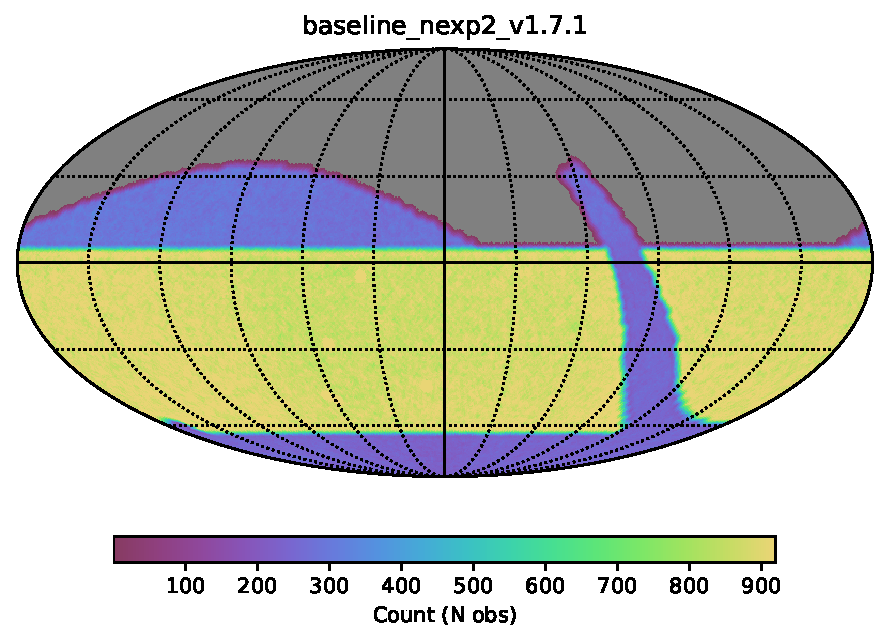
\includegraphics[height=1.25in, width=1.75in]{plots/baseline_nexp2_v1.7.1/baseline_nexp2_v1_7_1_Count_HEAL_SkyMap.pdf}
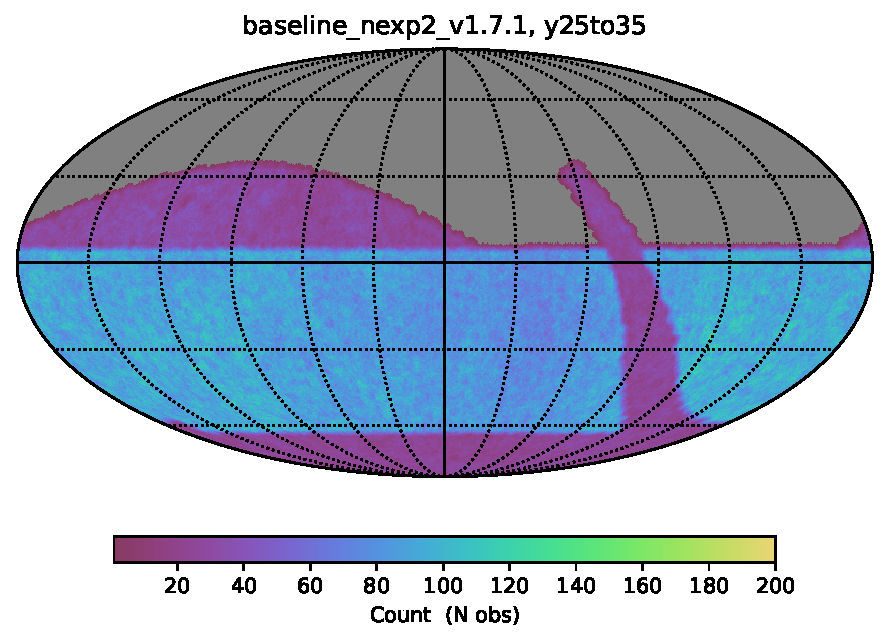
\includegraphics[height=1.25in, width=1.75in]{plots/baseline_nexp2_v1.7.1/baseline_nexp2_v1_7_1_Count_night_gt_913_125000_and_night_lt_1278_375000_and_note_not_like_DD_HEAL_SkyMap.pdf}
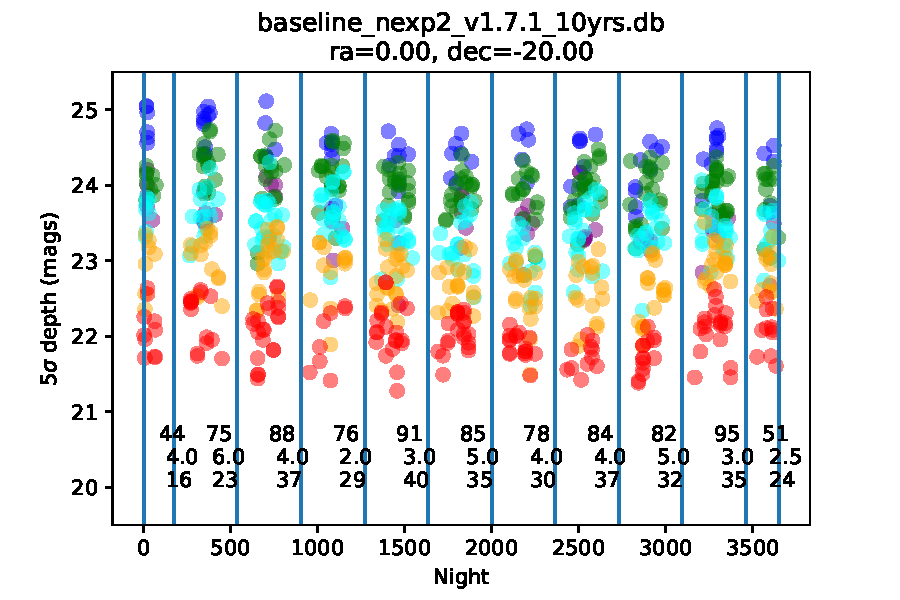
\includegraphics[height=1.25in, width=1.75in]{plots/baseline_nexp2_v171_spotc.pdf}\\
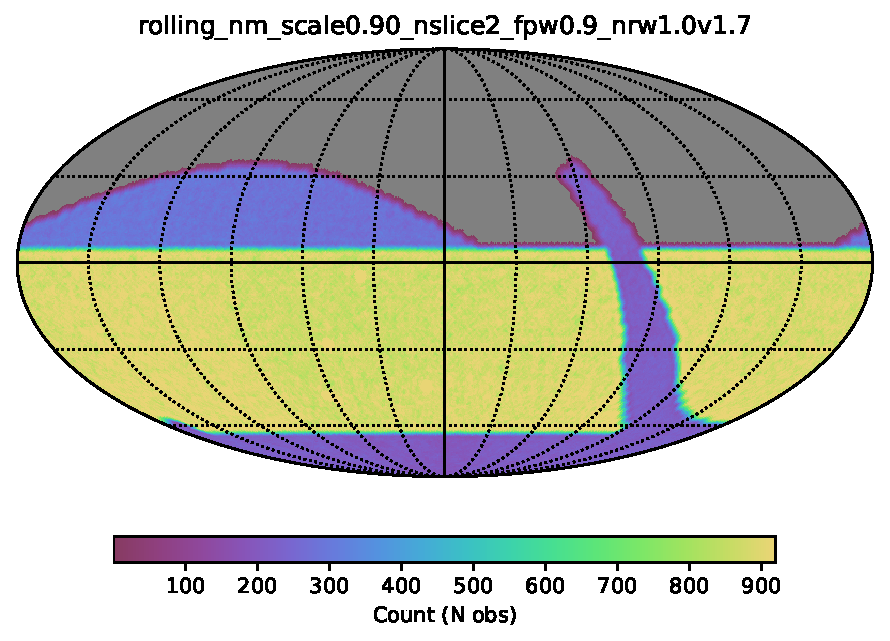
\includegraphics[height=1.25in, width=1.75in]{plots/rolling_nm_scale0.90_nslice2_fpw0.9_nrw1.0v1.7/rolling_nm_scale0_90_nslice2_fpw0_9_nrw1_0v1_7_Count_HEAL_SkyMap.pdf}
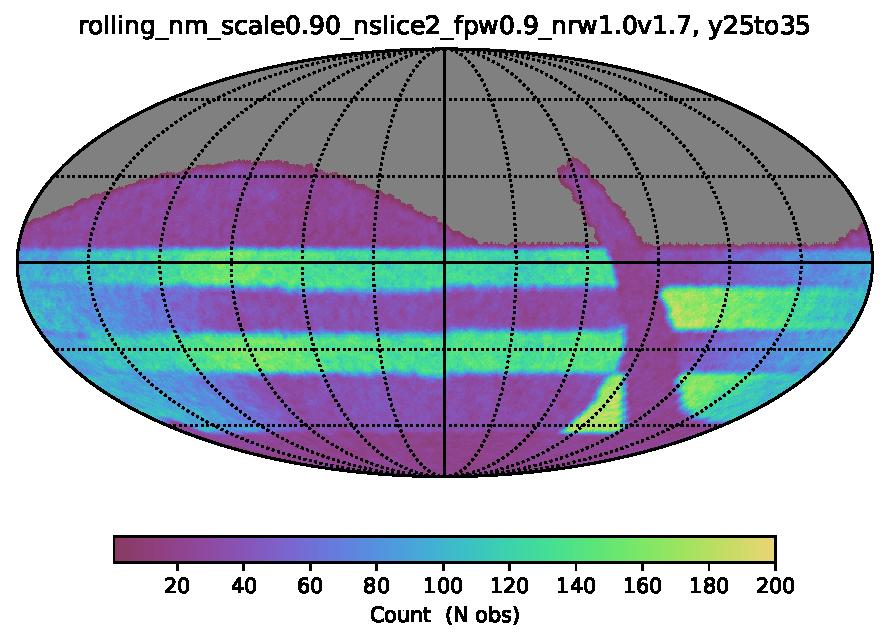
\includegraphics[height=1.25in, width=1.75in]{plots/rolling_nm_scale0.90_nslice2_fpw0.9_nrw1.0v1.7/rolling_nm_scale0_90_nslice2_fpw0_9_nrw1_0v1_7_Count_night_gt_913_125000_and_night_lt_1278_375000_and_note_not_like_DD_HEAL_SkyMap.pdf}
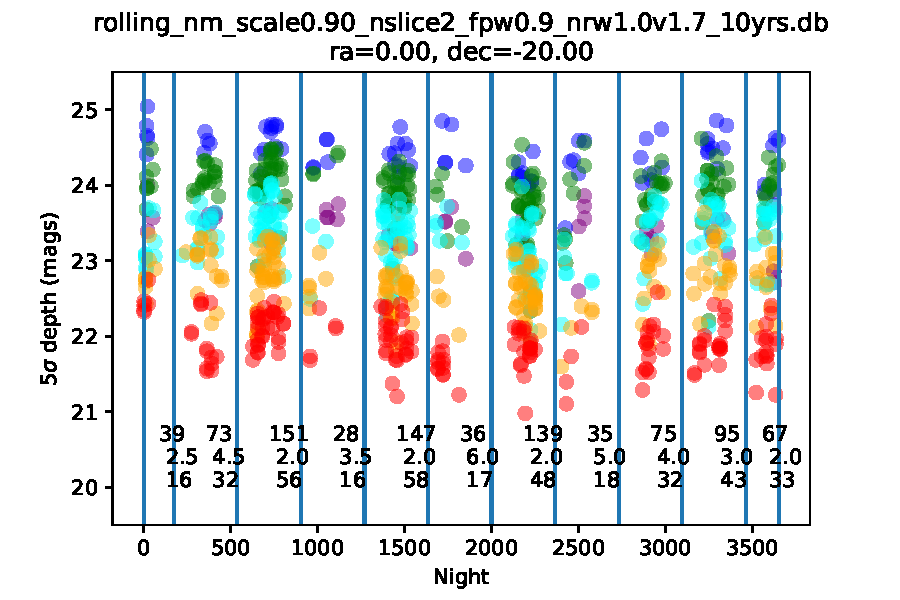
\includegraphics[height=1.25in, width=1.75in]{plots/rolling_nm_scale090_nslice2_fpw09_nrw10v17_spotc.pdf}\\
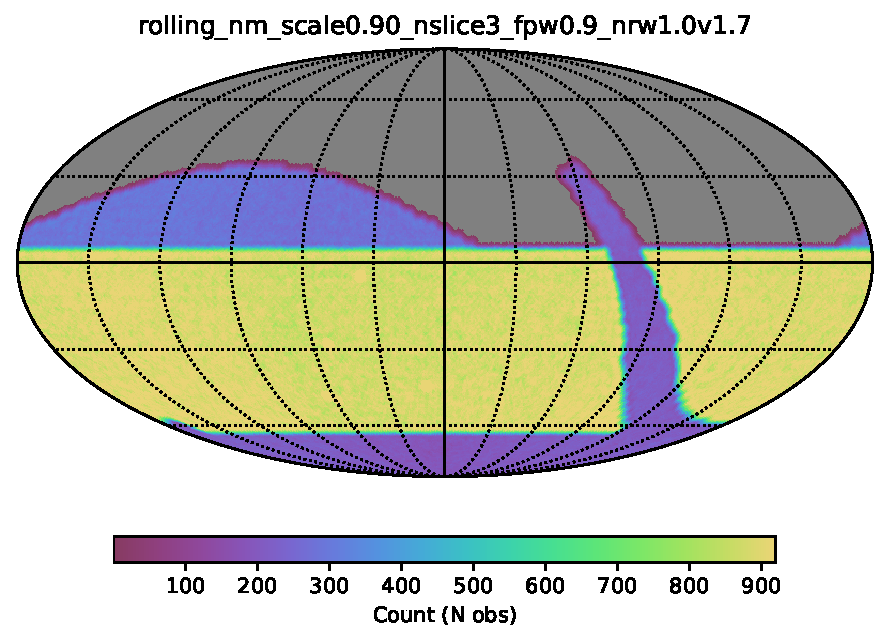
\includegraphics[height=1.25in, width=1.75in]{plots/rolling_nm_scale0.90_nslice3_fpw0.9_nrw1.0v1.7/rolling_nm_scale0_90_nslice3_fpw0_9_nrw1_0v1_7_Count_HEAL_SkyMap.pdf}
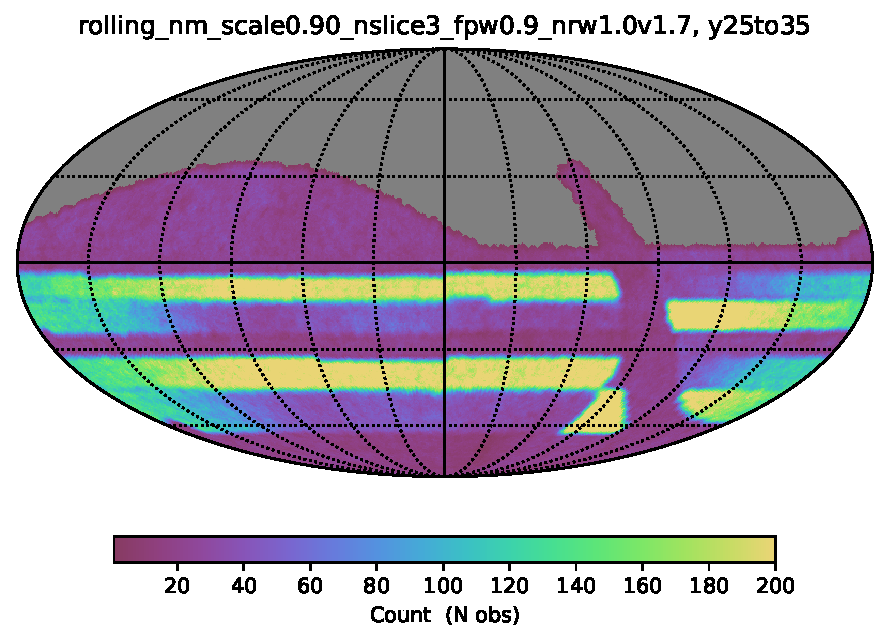
\includegraphics[height=1.25in, width=1.75in]{plots/rolling_nm_scale0.90_nslice3_fpw0.9_nrw1.0v1.7/rolling_nm_scale0_90_nslice3_fpw0_9_nrw1_0v1_7_Count_night_gt_913_125000_and_night_lt_1278_375000_and_note_not_like_DD_HEAL_SkyMap.pdf}
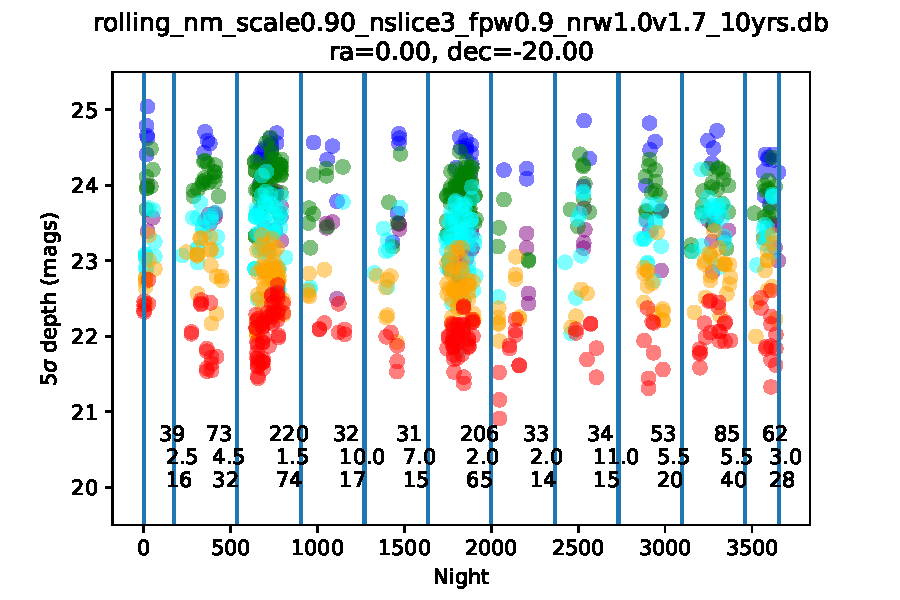
\includegraphics[height=1.25in, width=1.75in]{plots/rolling_nm_scale090_nslice3_fpw09_nrw10v17_spotc.pdf}
\caption{Plots showing the results for various simulations with the classic survey footprint. On the left, we plot the total number of observations (all filters) after 10 years. Middle panels show non-deep drilling observations taken between years 2.5 and 3.5. Right panels show observations that overlap a fiducial WFD point at RA=0, dec=-20. Horizontal lines denote different observing seasons, with annotations for the total number of observations in a season, median gap between days that have an observation, and the total number of unique days in the season with an observation. The top shows the baseline strategy, middle a rolling cadence where half the sky is rolling for three on and three off seasons, bottom shows a rolling cadence where one third of the sky is on for two seasons and off for four seasons. The full-sky randomized nightly dithering does an excellent job, leaving no trace of the declination banding in the final 10 year rolling simulations. \label{fig:classics}}
\end{figure}



\begin{figure}
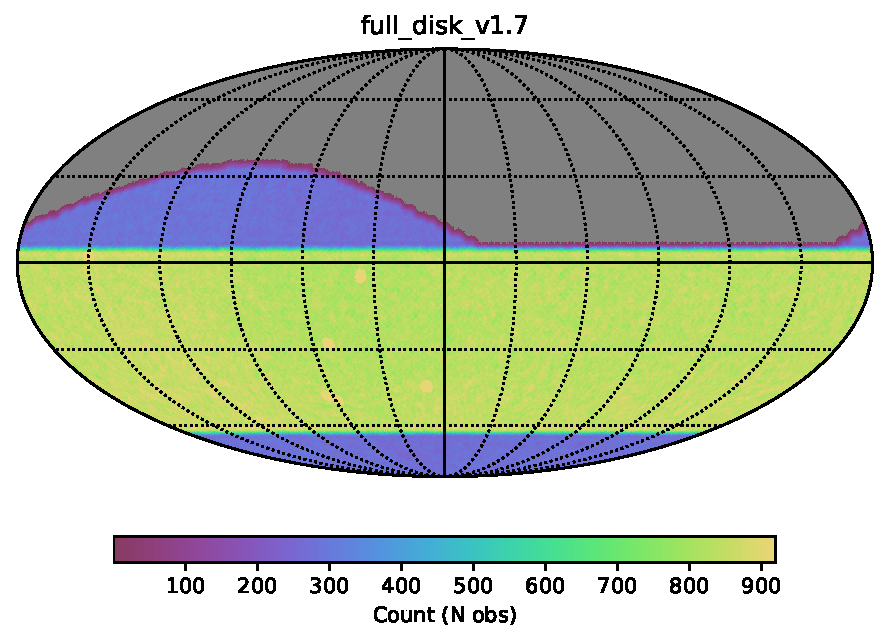
\includegraphics[height=1.25in, width=1.75in]{plots/full_disk_v1.7/full_disk_v1_7_Count_HEAL_SkyMap.pdf}
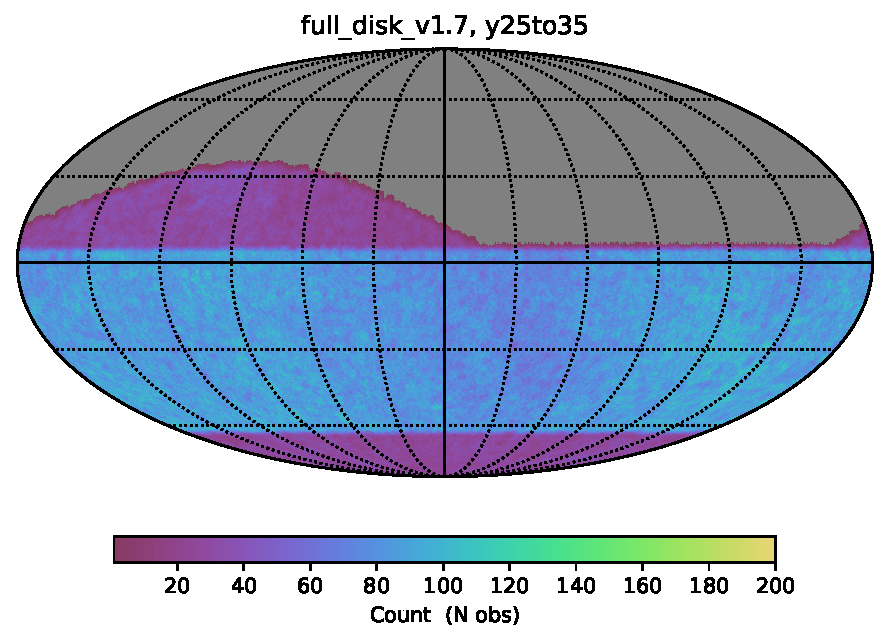
\includegraphics[height=1.25in, width=1.75in]{plots/full_disk_v1.7/full_disk_v1_7_Count_night_gt_913_125000_and_night_lt_1278_375000_and_note_not_like_DD_HEAL_SkyMap.pdf}
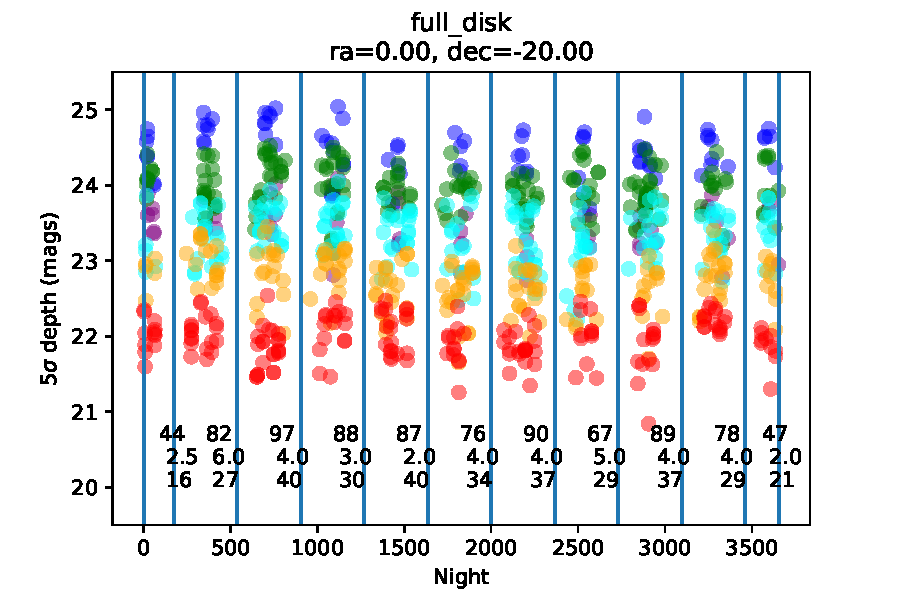
\includegraphics[height=1.25in, width=1.75in]{plots/full_disk_v17_spotc.pdf} \\
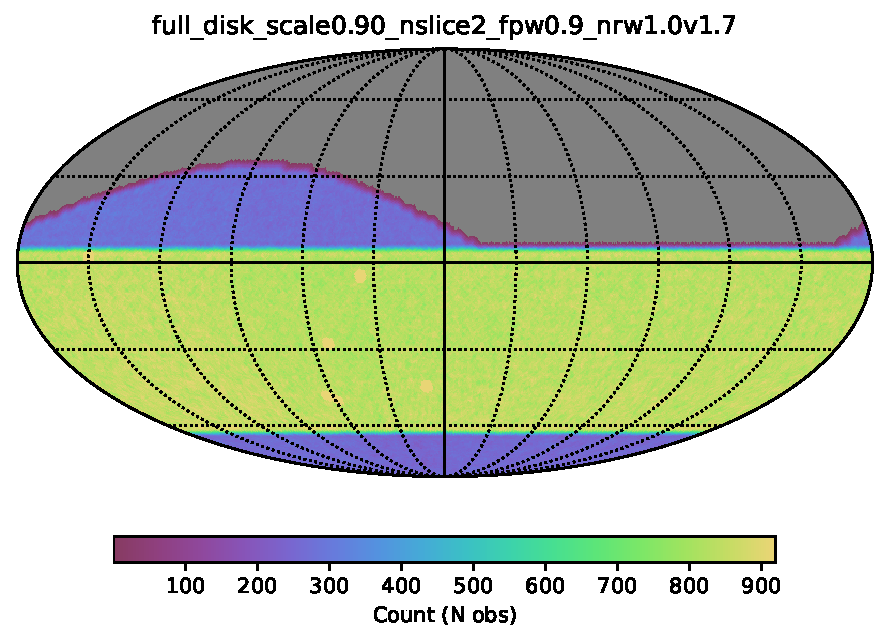
\includegraphics[height=1.25in, width=1.75in]{plots/full_disk_scale0.90_nslice2_fpw0.9_nrw1.0v1.7/full_disk_scale0_90_nslice2_fpw0_9_nrw1_0v1_7_Count_HEAL_SkyMap.pdf}
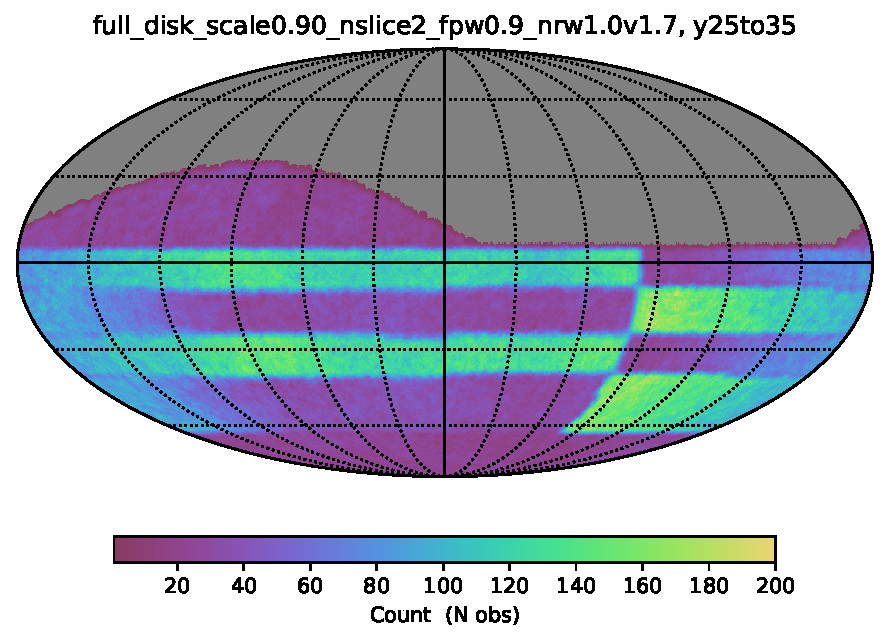
\includegraphics[height=1.25in, width=1.75in]{plots/full_disk_scale0.90_nslice2_fpw0.9_nrw1.0v1.7/full_disk_scale0_90_nslice2_fpw0_9_nrw1_0v1_7_Count_night_gt_913_125000_and_night_lt_1278_375000_and_note_not_like_DD_HEAL_SkyMap.pdf}
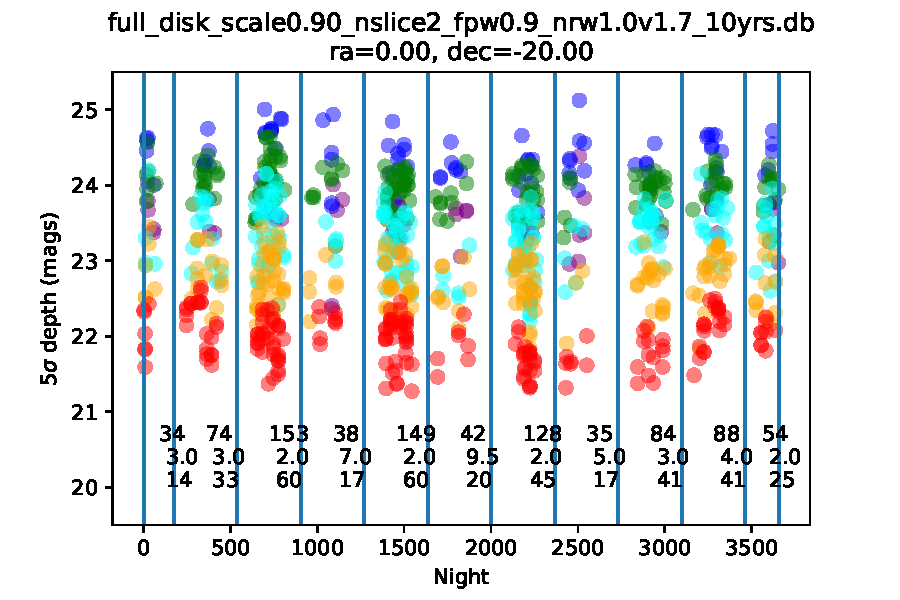
\includegraphics[height=1.25in, width=1.75in]{plots/full_disk_scale090_nslice2_fpw09_nrw10v17_spotc.pdf} \\
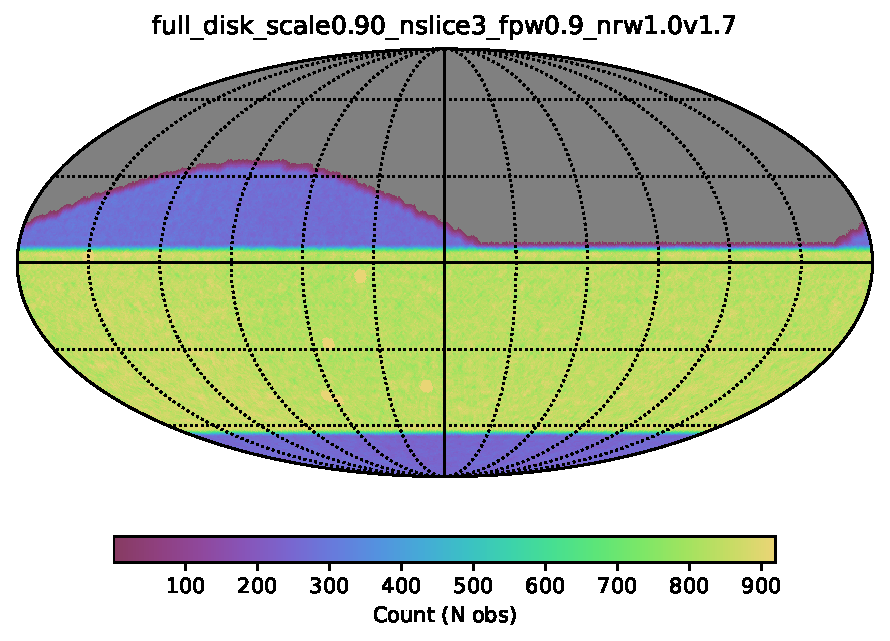
\includegraphics[height=1.25in, width=1.75in]{plots/full_disk_scale0.90_nslice3_fpw0.9_nrw1.0v1.7/full_disk_scale0_90_nslice3_fpw0_9_nrw1_0v1_7_Count_HEAL_SkyMap.pdf}
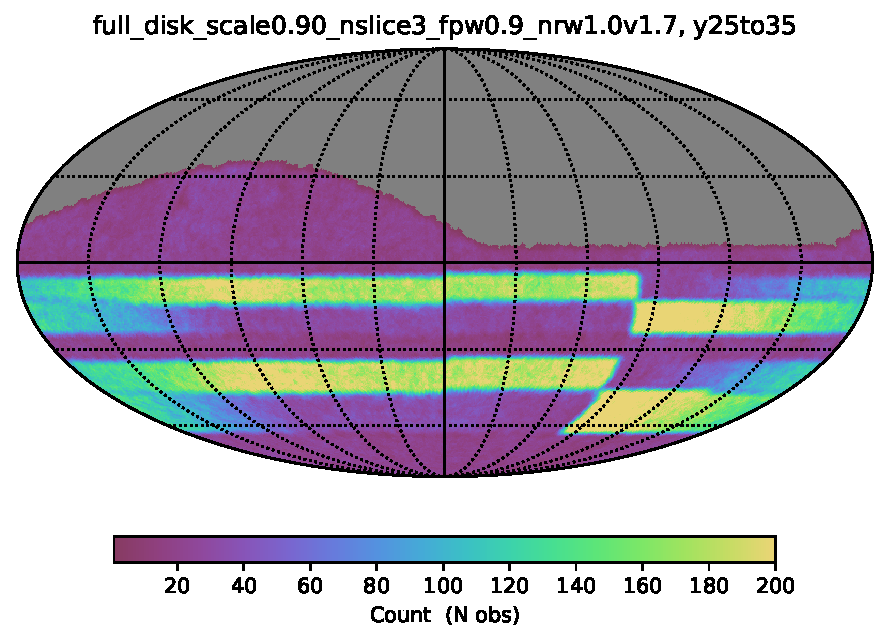
\includegraphics[height=1.25in, width=1.75in]{plots/full_disk_scale0.90_nslice3_fpw0.9_nrw1.0v1.7/full_disk_scale0_90_nslice3_fpw0_9_nrw1_0v1_7_Count_night_gt_913_125000_and_night_lt_1278_375000_and_note_not_like_DD_HEAL_SkyMap.pdf}
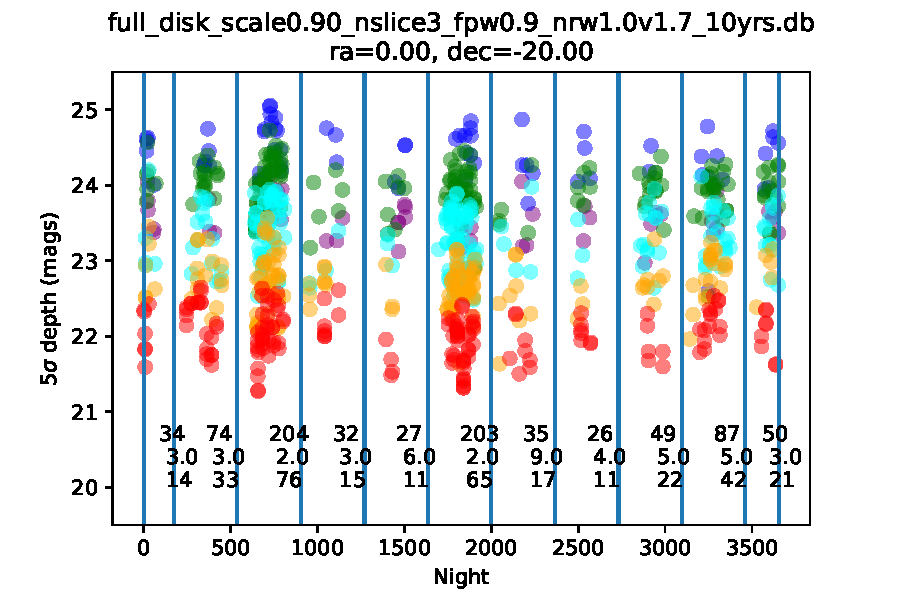
\includegraphics[height=1.25in, width=1.75in]{plots/full_disk_scale090_nslice3_fpw09_nrw10v17_spotc.pdf}
\caption{Like Figure~\ref{fig:classics} but for a footprint that treats the Galactic plane as part of the WFD region. \label{fig:fulldisk}}
\end{figure}


\begin{figure}
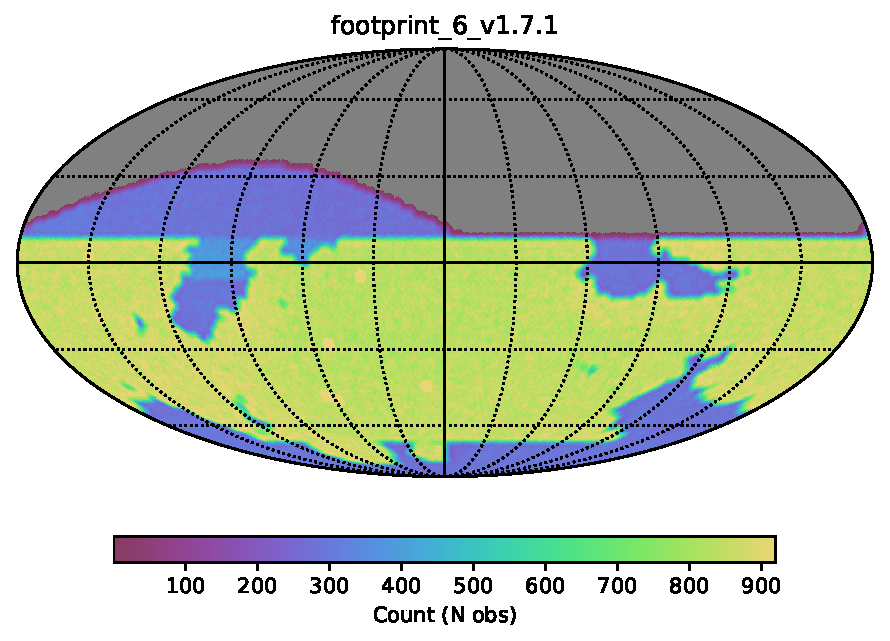
\includegraphics[height=1.25in, width=1.75in]{plots/footprint_6_v1.7.1/footprint_6_v1_7_1_Count_HEAL_SkyMap.pdf}
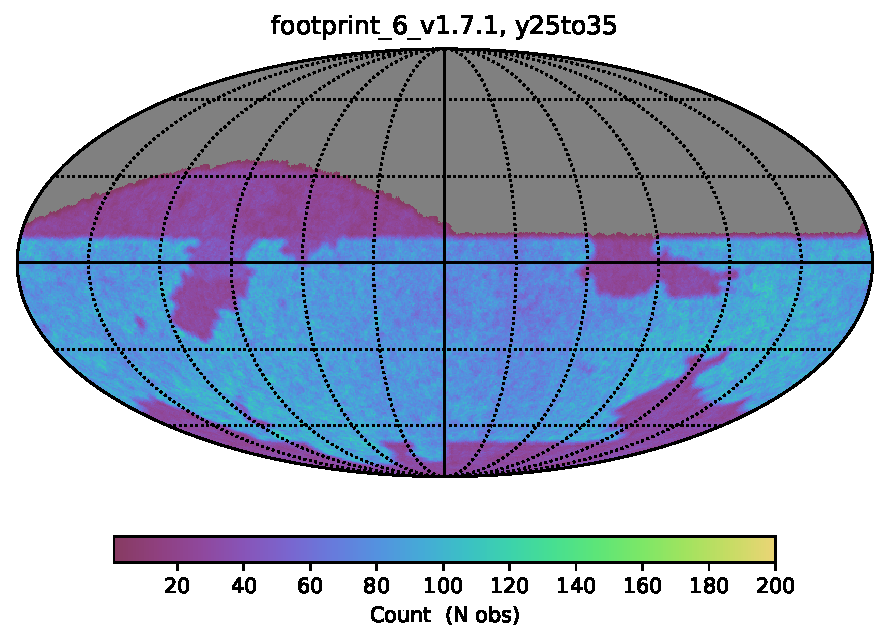
\includegraphics[height=1.25in, width=1.75in]{plots/footprint_6_v1.7.1/footprint_6_v1_7_1_Count_night_gt_913_125000_and_night_lt_1278_375000_and_note_not_like_DD_HEAL_SkyMap.pdf}
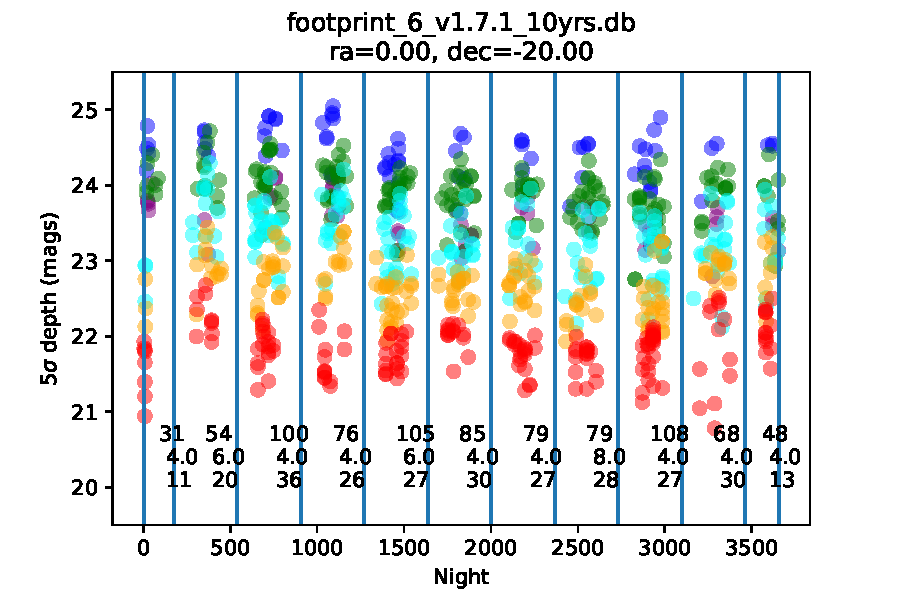
\includegraphics[height=1.25in, width=1.75in]{plots/footprint_6_v171_spotc.pdf} \\

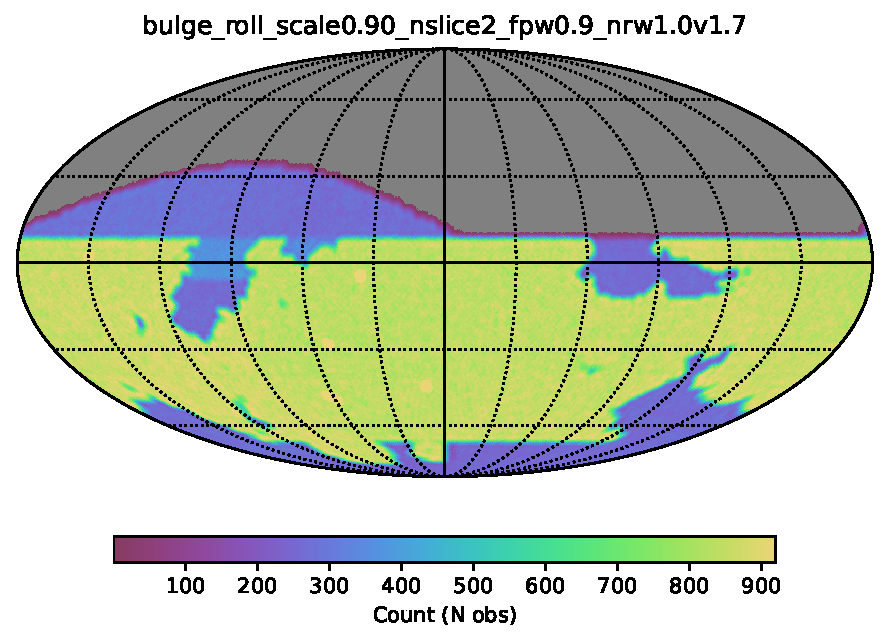
\includegraphics[height=1.25in, width=1.75in]{plots/bulge_roll_scale0.90_nslice2_fpw0.9_nrw1.0v1.7/bulge_roll_scale0_90_nslice2_fpw0_9_nrw1_0v1_7_Count_HEAL_SkyMap.pdf}
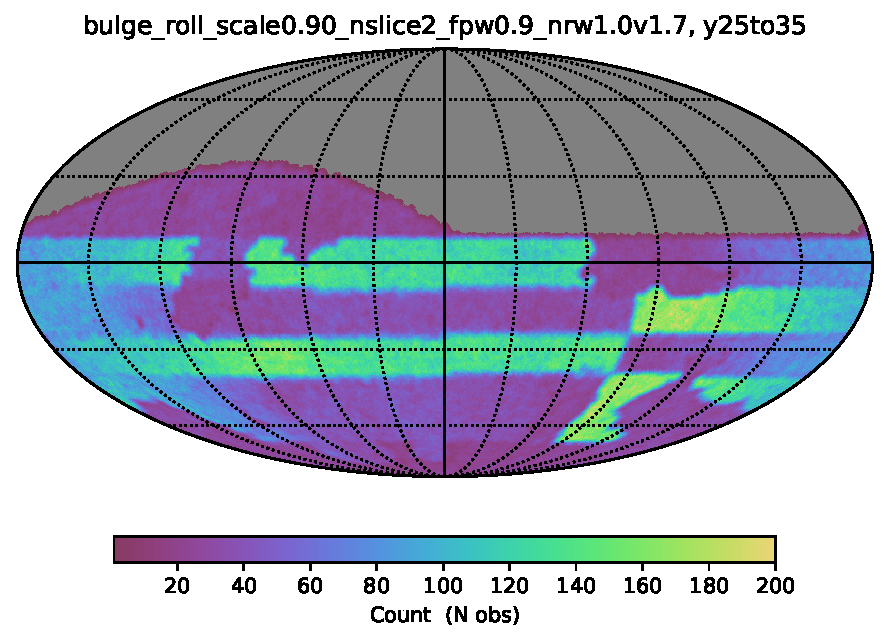
\includegraphics[height=1.25in, width=1.75in]{plots/bulge_roll_scale0.90_nslice2_fpw0.9_nrw1.0v1.7/bulge_roll_scale0_90_nslice2_fpw0_9_nrw1_0v1_7_Count_night_gt_913_125000_and_night_lt_1278_375000_and_note_not_like_DD_HEAL_SkyMap.pdf}
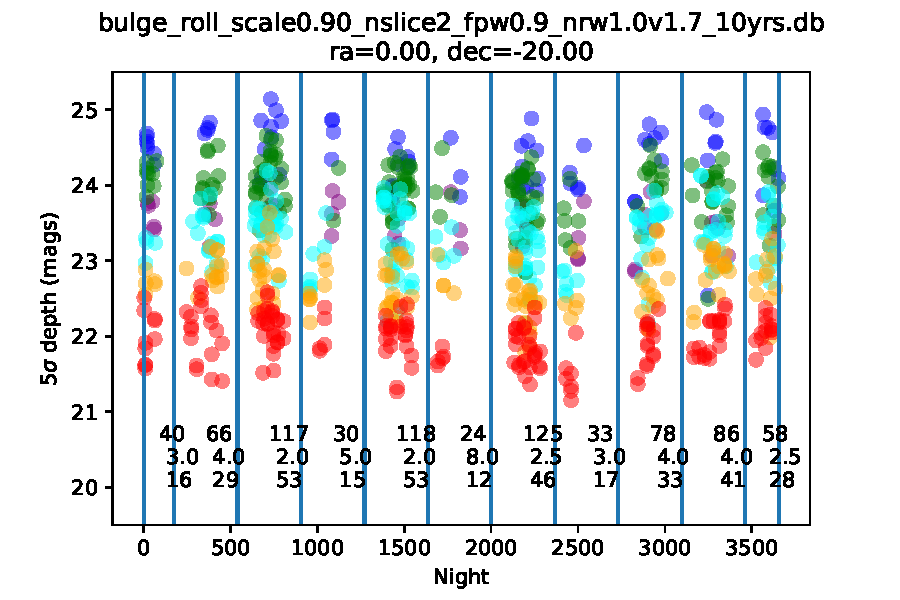
\includegraphics[height=1.25in, width=1.75in]{plots/bulge_roll_scale090_nslice2_fpw09_nrw10v17_spotc.pdf} \\
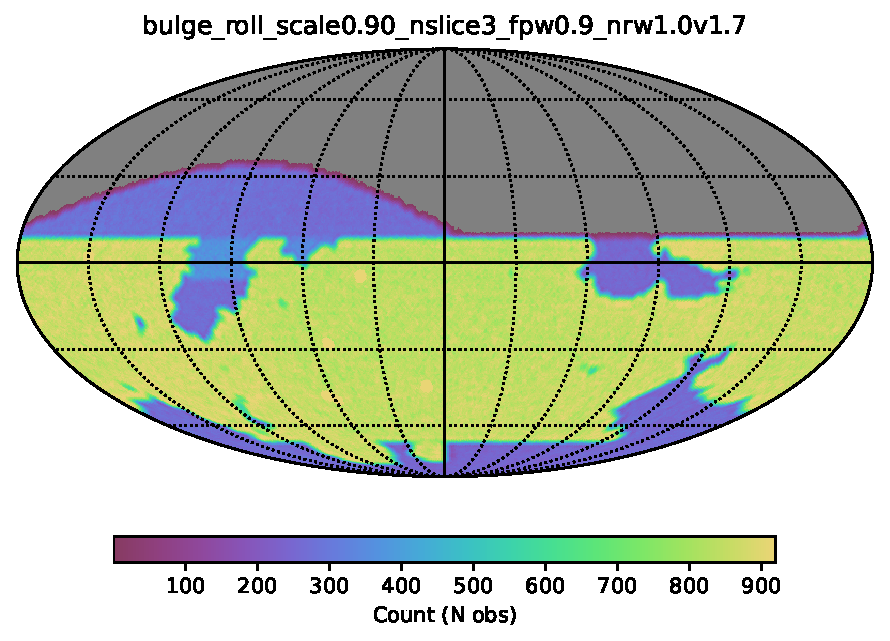
\includegraphics[height=1.25in, width=1.75in]{plots/bulge_roll_scale0.90_nslice3_fpw0.9_nrw1.0v1.7/bulge_roll_scale0_90_nslice3_fpw0_9_nrw1_0v1_7_Count_HEAL_SkyMap.pdf}
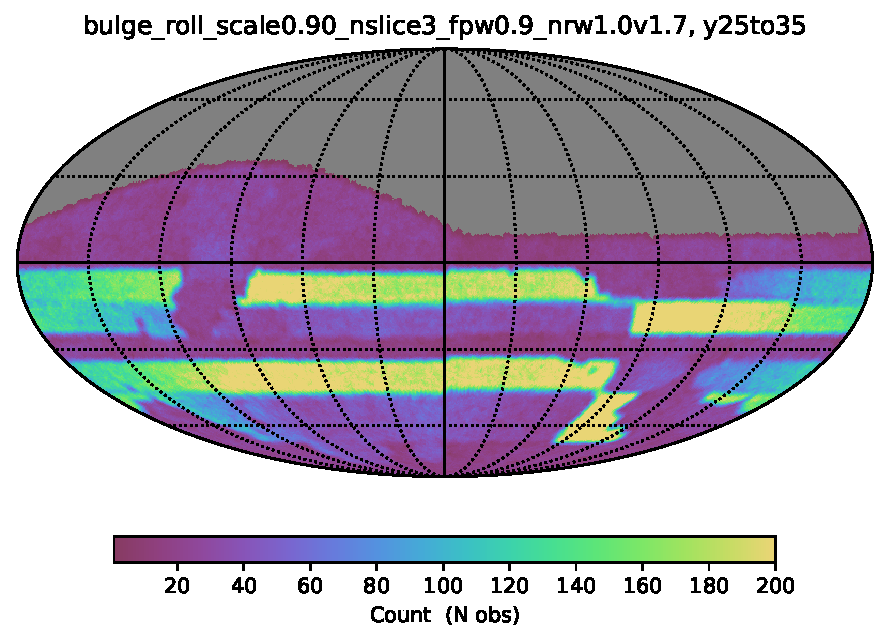
\includegraphics[height=1.25in, width=1.75in]{plots/bulge_roll_scale0.90_nslice3_fpw0.9_nrw1.0v1.7/bulge_roll_scale0_90_nslice3_fpw0_9_nrw1_0v1_7_Count_night_gt_913_125000_and_night_lt_1278_375000_and_note_not_like_DD_HEAL_SkyMap.pdf}
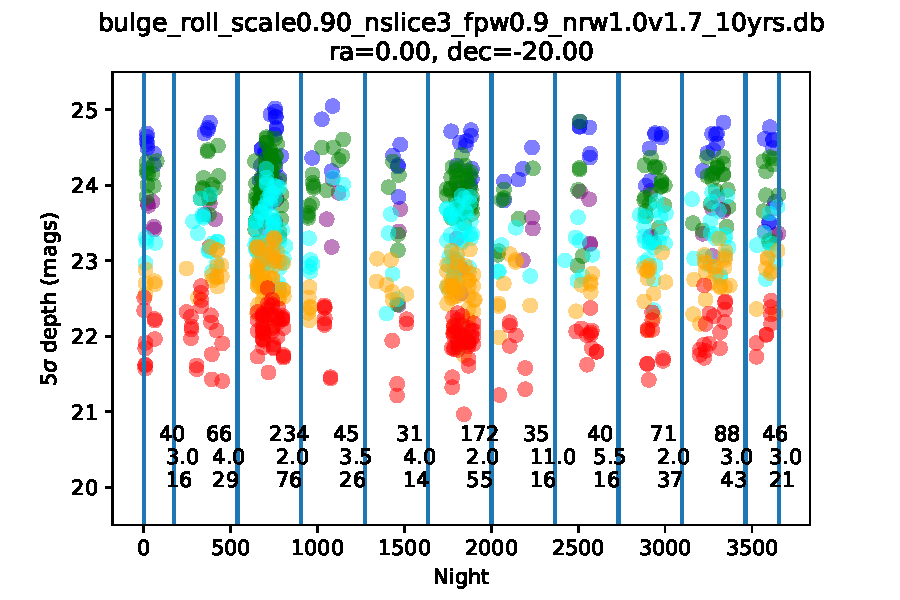
\includegraphics[height=1.25in, width=1.75in]{plots/bulge_roll_scale090_nslice3_fpw09_nrw10v17_spotc.pdf} \\
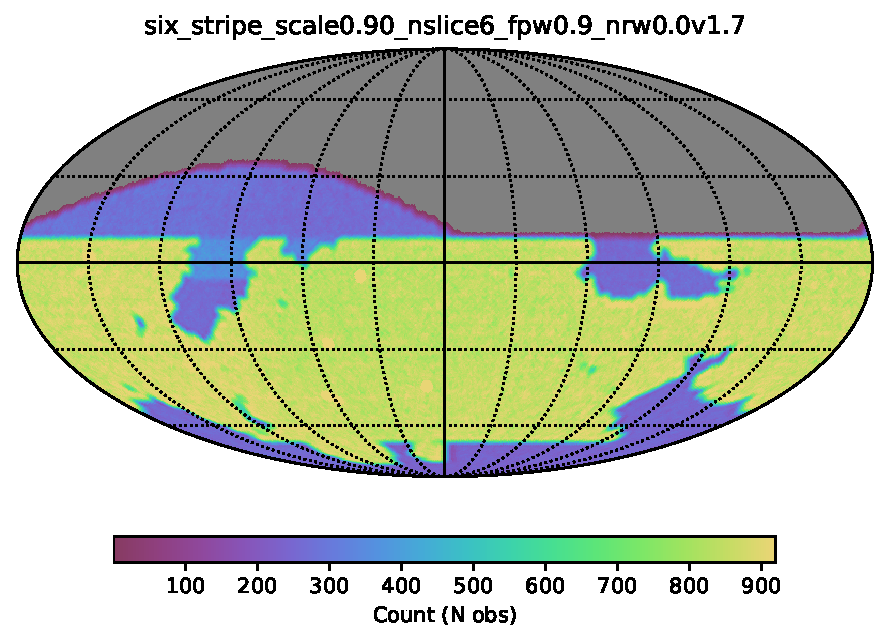
\includegraphics[height=1.25in, width=1.75in]{plots/six_stripe_scale0.90_nslice6_fpw0.9_nrw0.0v1.7/six_stripe_scale0_90_nslice6_fpw0_9_nrw0_0v1_7_Count_HEAL_SkyMap.pdf}
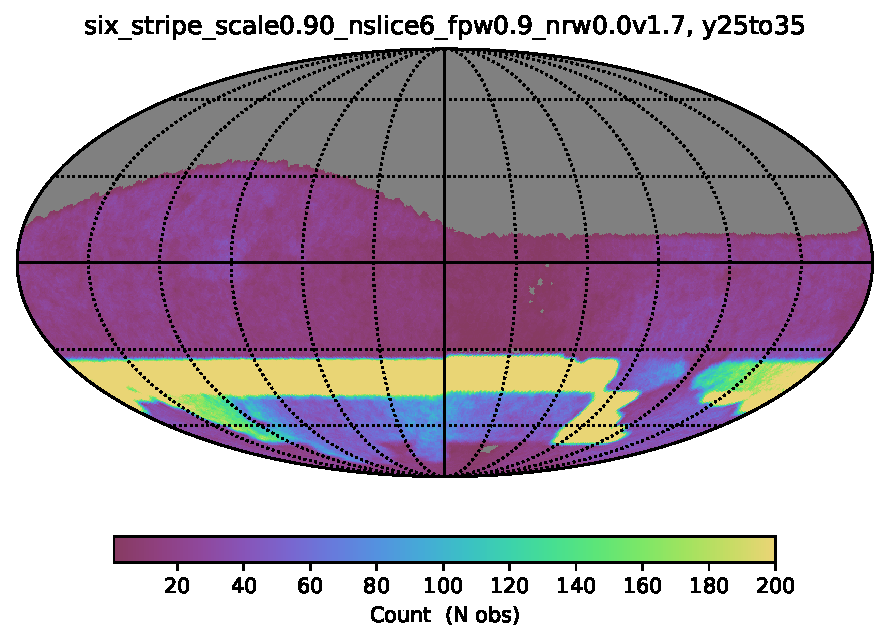
\includegraphics[height=1.25in, width=1.75in]{plots/six_stripe_scale0.90_nslice6_fpw0.9_nrw0.0v1.7/six_stripe_scale0_90_nslice6_fpw0_9_nrw0_0v1_7_Count_night_gt_913_125000_and_night_lt_1278_375000_and_note_not_like_DD_HEAL_SkyMap.pdf}
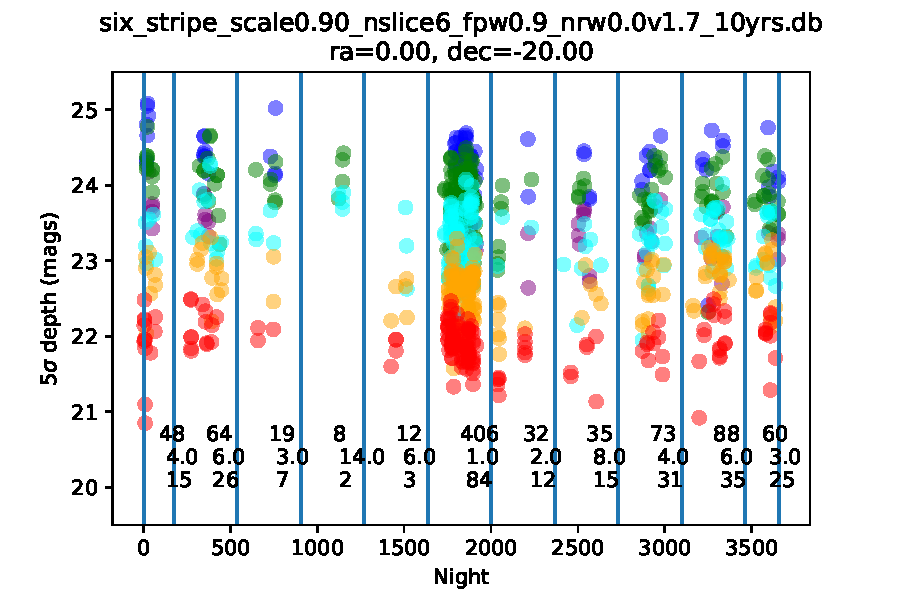
\includegraphics[height=1.25in, width=1.75in]{plots/six_stripe_scale090_nslice6_fpw09_nrw00v17_spotc.pdf}
\caption{Like Figure~\ref{fig:classics}, but for a compromise footprint that includes the bulge, a plane bridge, and the Magellanic Clouds as part of WFD. Here we have also included an extreme rolling with 6 bands. This results in a point on the sky having one high cadence season and 5 low cadence seasons. Note that such extreme rolling means that there will be multiple years where northern telescopes have little to no chance to follow up Rubin alerts. \label{fig:compsky}}
\end{figure}




\begin{figure}
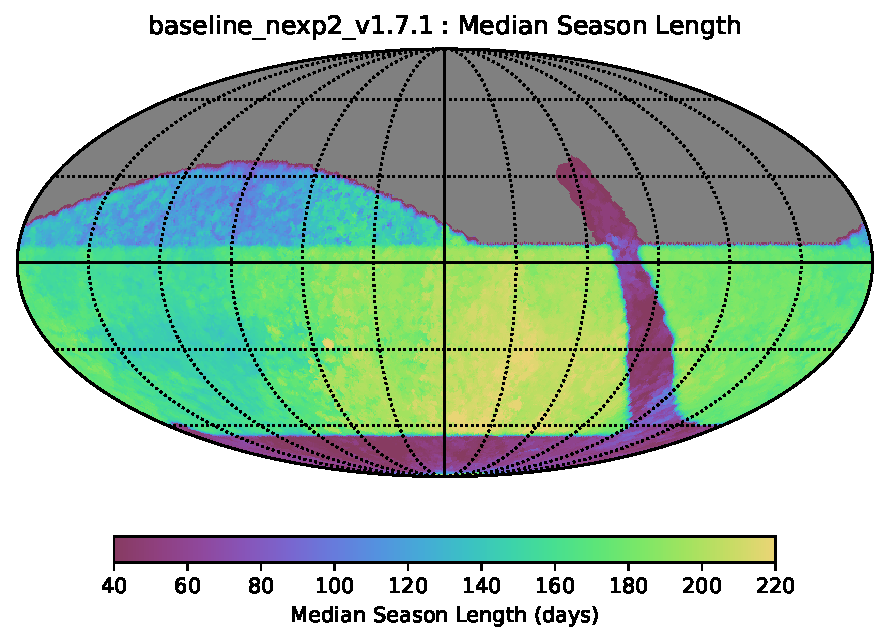
\includegraphics[width=1.75in]{plots/seasons/baseline_nexp2_v1_7_1_Median_Season_Length_HEAL_SkyMap.pdf}
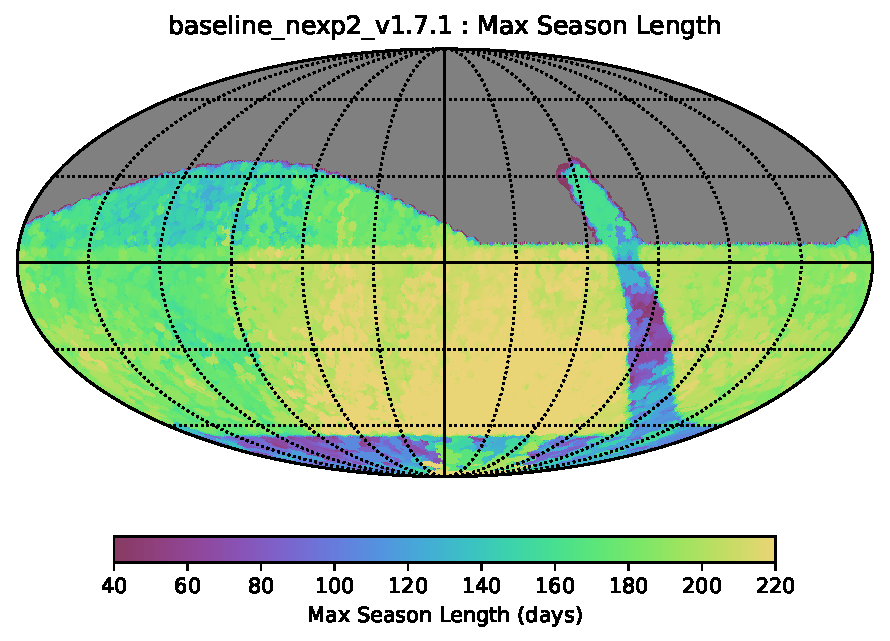
\includegraphics[width=1.75in]{plots/seasons/baseline_nexp2_v1_7_1_Max_Season_Length_HEAL_SkyMap.pdf}
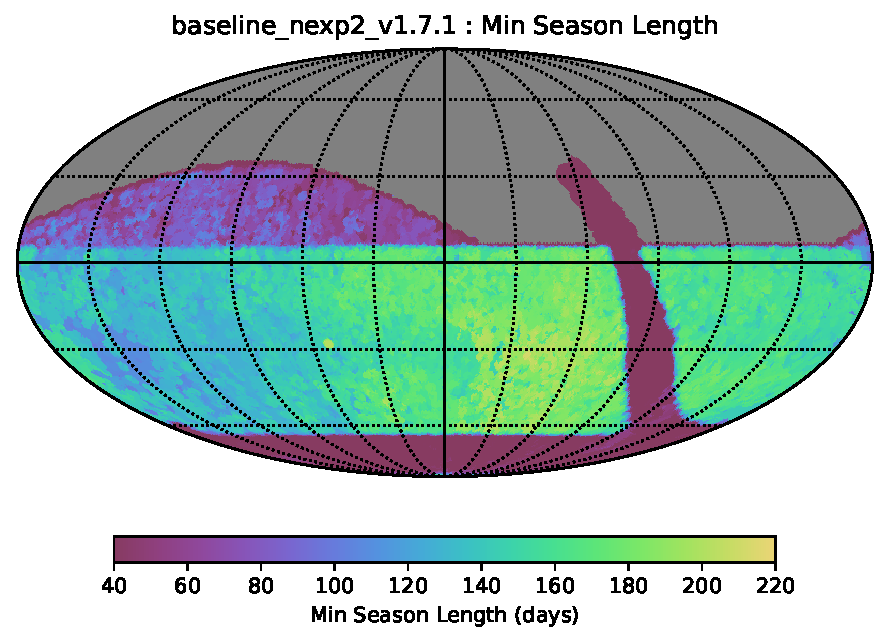
\includegraphics[width=1.75in]{plots/seasons/baseline_nexp2_v1_7_1_Min_Season_Length_HEAL_SkyMap.pdf} \\
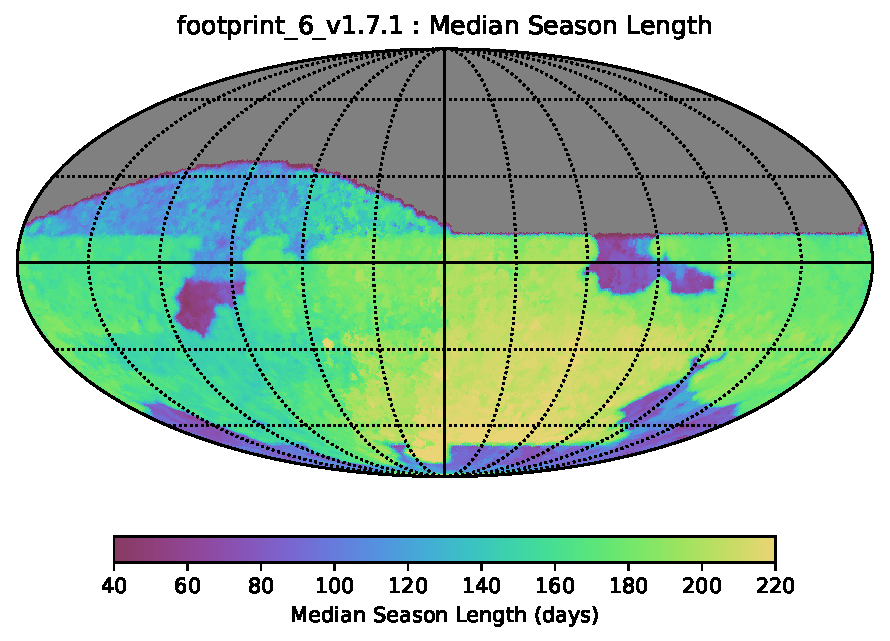
\includegraphics[width=1.75in]{plots/seasons/footprint_6_v1_7_1_Median_Season_Length_HEAL_SkyMap.pdf}
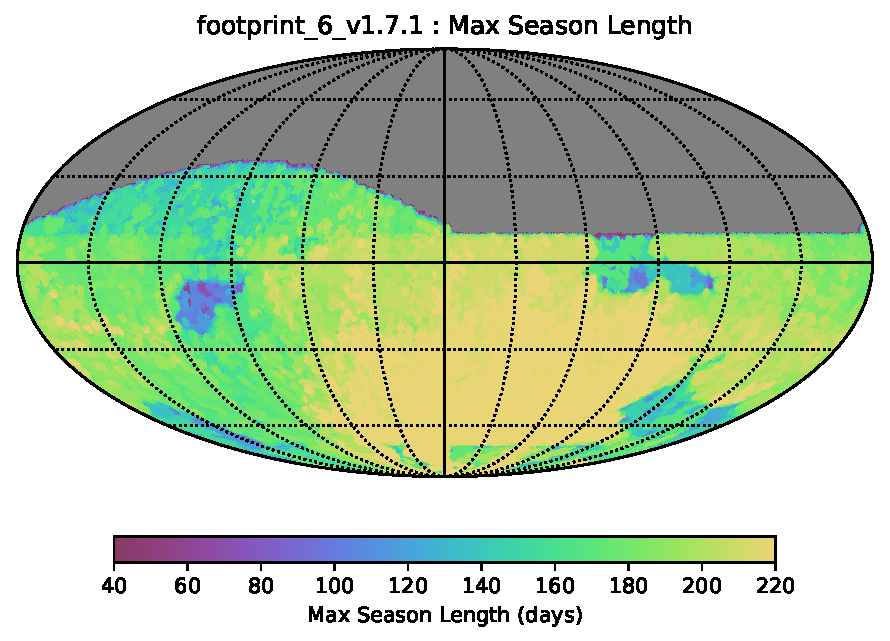
\includegraphics[width=1.75in]{plots/seasons/footprint_6_v1_7_1_Max_Season_Length_HEAL_SkyMap.pdf}
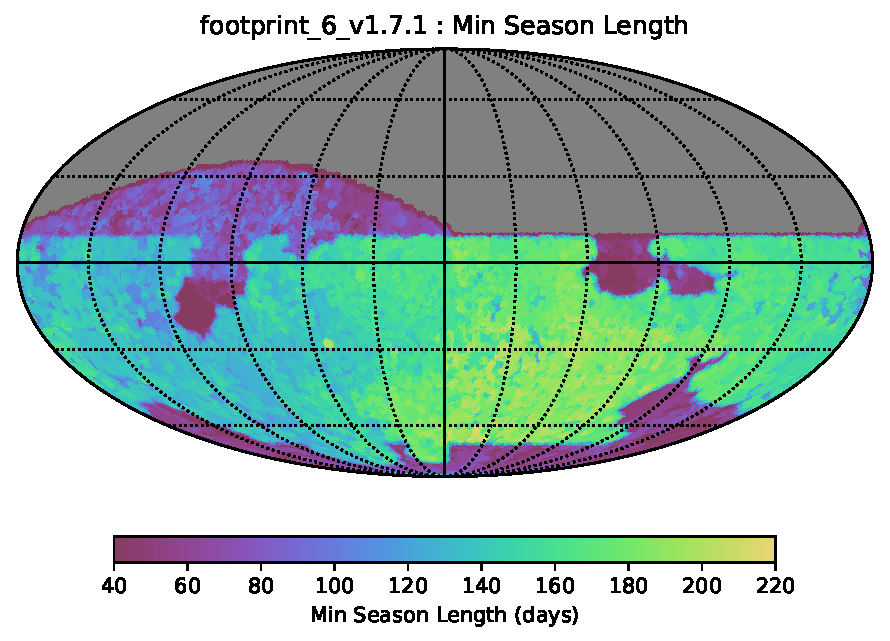
\includegraphics[width=1.75in]{plots/seasons/footprint_6_v1_7_1_Min_Season_Length_HEAL_SkyMap.pdf} \\
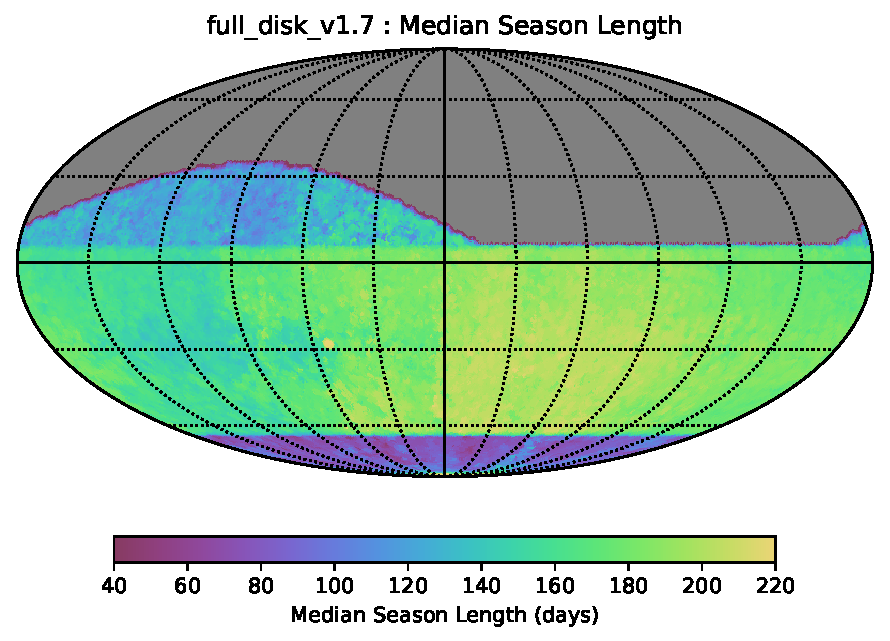
\includegraphics[width=1.75in]{plots/seasons/full_disk_v1_7_Median_Season_Length_HEAL_SkyMap.pdf}
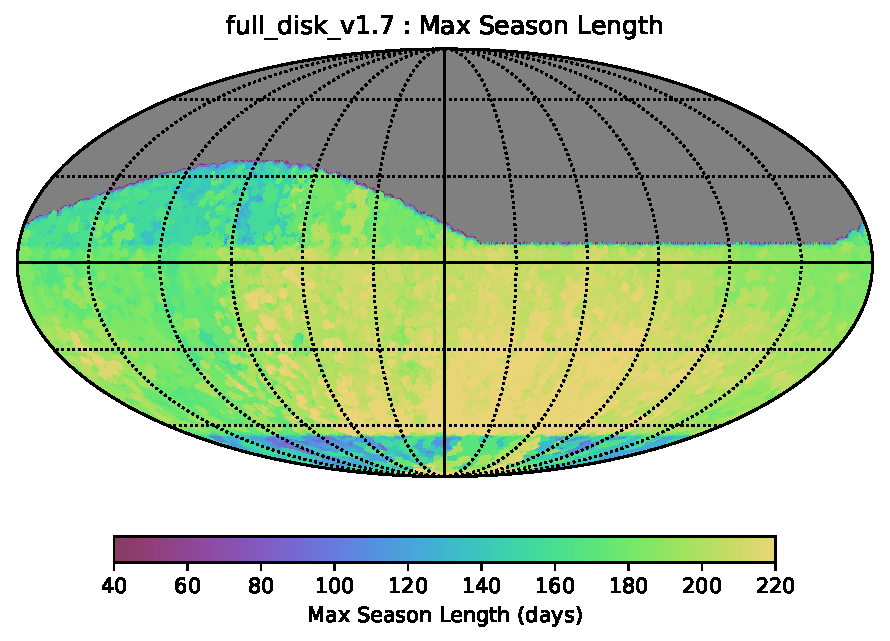
\includegraphics[width=1.75in]{plots/seasons/full_disk_v1_7_Max_Season_Length_HEAL_SkyMap.pdf}
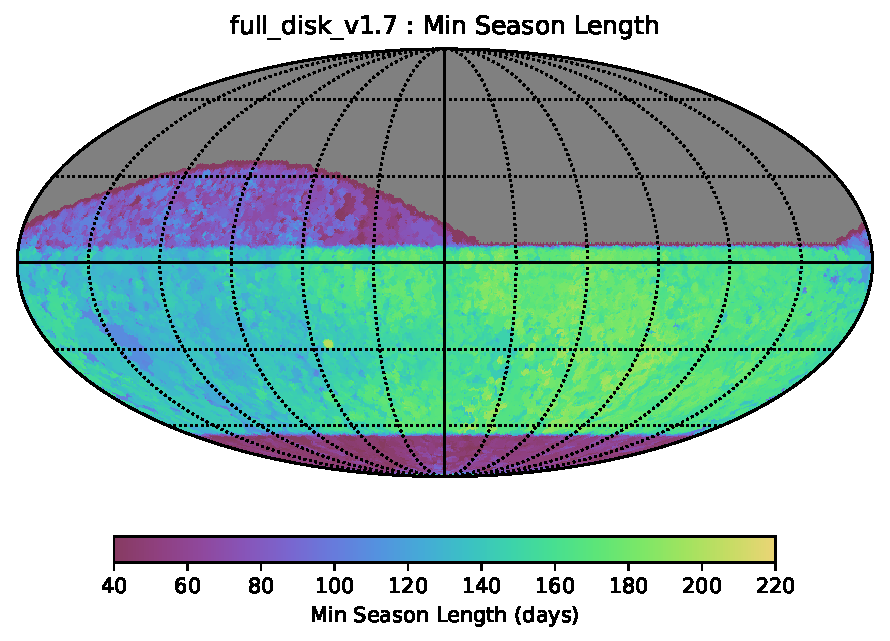
\includegraphics[width=1.75in]{plots/seasons/full_disk_v1_7_Min_Season_Length_HEAL_SkyMap.pdf}
\caption{The median, max, and minimum season length for the non-rolling simulations (excluding the first and last seasons). While the footprint object uses a nominal season length of 183 days, the scheduler must compensate for regions of sky that are over and under subscribed to maintain survey uniformity. This results in gradients in the seasons lengths across the sky.}
\end{figure}



\begin{table}
\begin{tabular}{lccccc}\label{tab:metrics}

 Run Name &  SNe &  Fast Microlensing &  Slow Microlensing &  Max in season &  Min in season \\
 &           N    & Fraction  & Fraction     &   Number & at RA,dec=0,-20 \\
\toprule

baseline\_nexp2 &              22879.30 &                    0.15 &                    0.95 &     95 &     75 \\
rolling\_nslice2 &             29020.63 &                    0.15 &                    0.95 &    151 &     28 \\
rolling\_nslice3 &             28971.53 &                    0.16 &                    0.95 &    220 &     31 \\

\hline
full\_disk &                      19965.27 &                    0.44 &                    0.95 &     97 &     67 \\
full\_disk\_nslice2 &             27043.85 &                    0.42 &                    0.95 &    153 &     35 \\
full\_disk\_nslice3 &             27473.19 &                    0.39 &                    0.95 &    204 &     26 \\

\hline
footprint\_6 &                     17817.33 &                    0.44 &                    0.95 &    108 &     54 \\
bulge\_roll\_nslice2 &             29456.26 &                    0.42 &                    0.95 &    125 &     24 \\
bulge\_roll\_nslice3 &             29754.55 &                    0.40 &                    0.95 &    234 &     31 \\
six\_stripe\_nslice6 &             30850.44 &                    0.34 &                    0.95 &    406 &      8 \\
\hline
\end{tabular}
\end{table}


\section{Implementation Details}


In the baseline, when pointings are selected for observation we demand the area be contiguous. For the rolling cadence runs, we relax this condition so the selected pointings can span multiple declination stripes if they need to.  We introduce a basis function that suppresses the reward for areas on the sky that have already been observed twice in a night (except for the 6-slice rolling where same night observations are allowed).

What about a year with bad weather? There is concern that if we have good weather in the first year of rolling, and then poor weather the next, something bad will happen. In this case, we expect the scheduler will compensate the next year to get back on schedule either by rolling slightly less, or using a year that would have normally been uniform to psudo-roll and return the survey to uniformity. With 2.5 years of uniform cadence at the end of the survey, we have plenty of time to recover from particularly bad weather years.



\section{Potential Shortcomings}

\begin{figure}
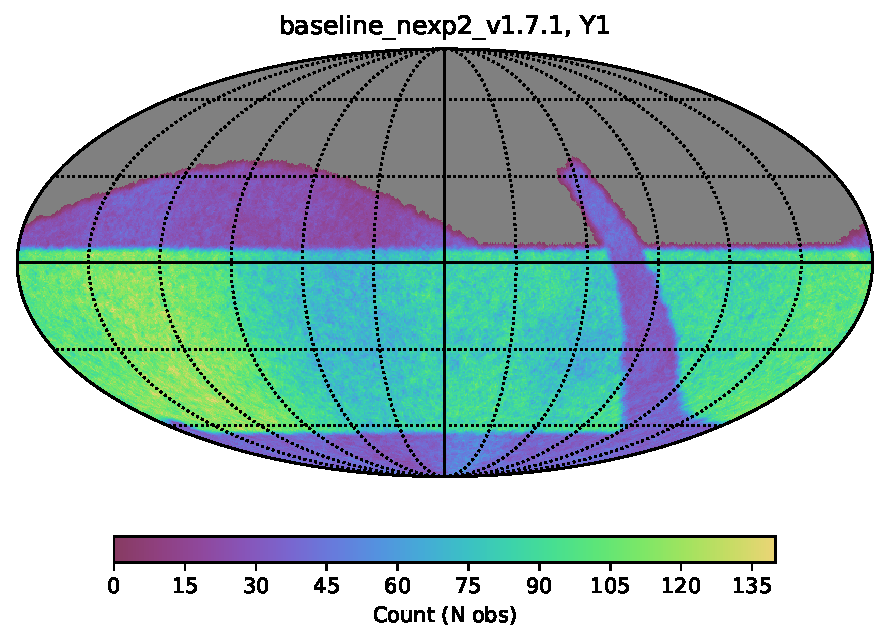
\includegraphics[width=1.75in]{plots/yearly_release/baseline_nexp2_v1_7_1_Count_night_lt_365_and_note_not_like_DD_HEAL_SkyMap.pdf}
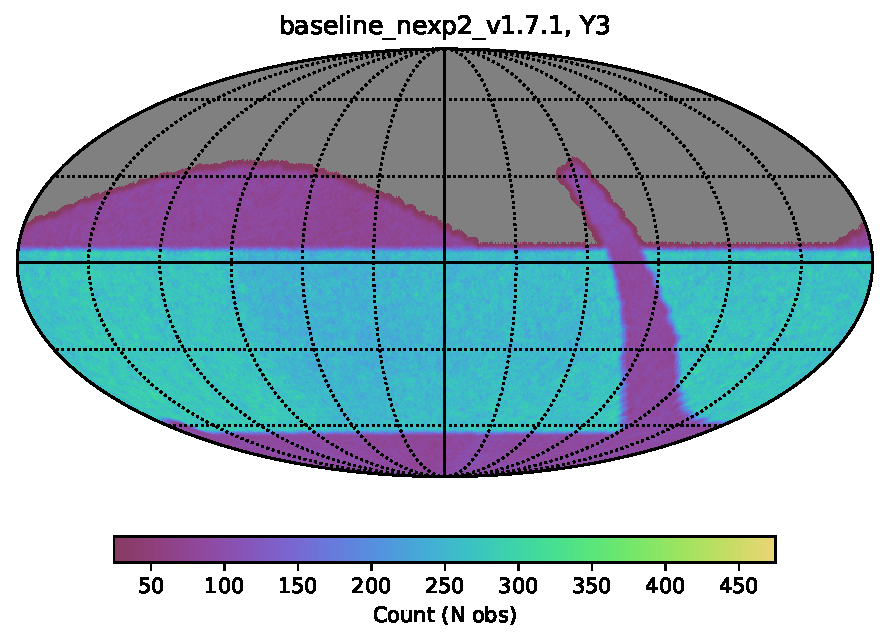
\includegraphics[width=1.75in]{plots/yearly_release/baseline_nexp2_v1_7_1_Count_nightlt1095_and_note_not_like_DD_HEAL_SkyMap.pdf}
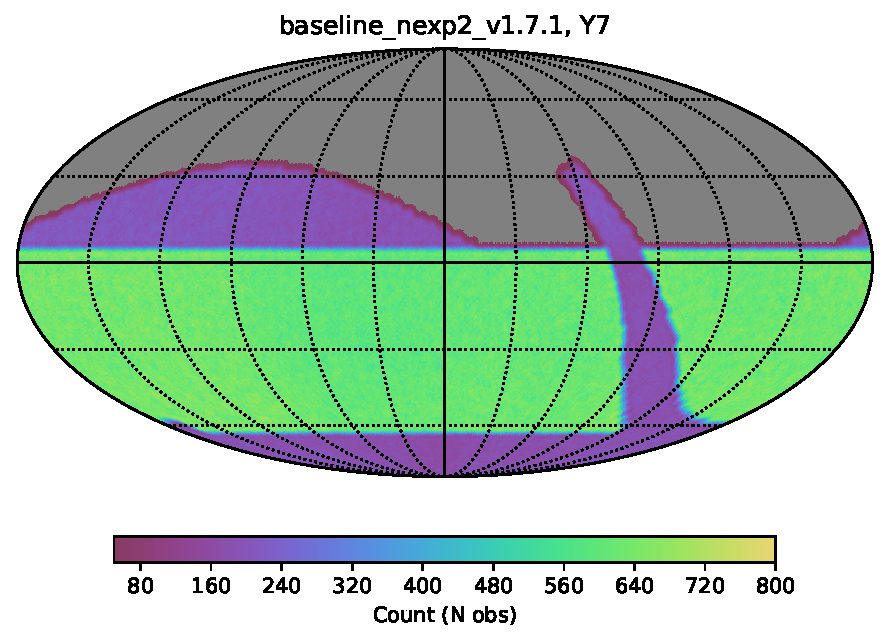
\includegraphics[width=1.75in]{plots/yearly_release/baseline_nexp2_v1_7_1_Count_night_lt_2556_and_note_not_like_DD_HEAL_SkyMap.pdf}\\
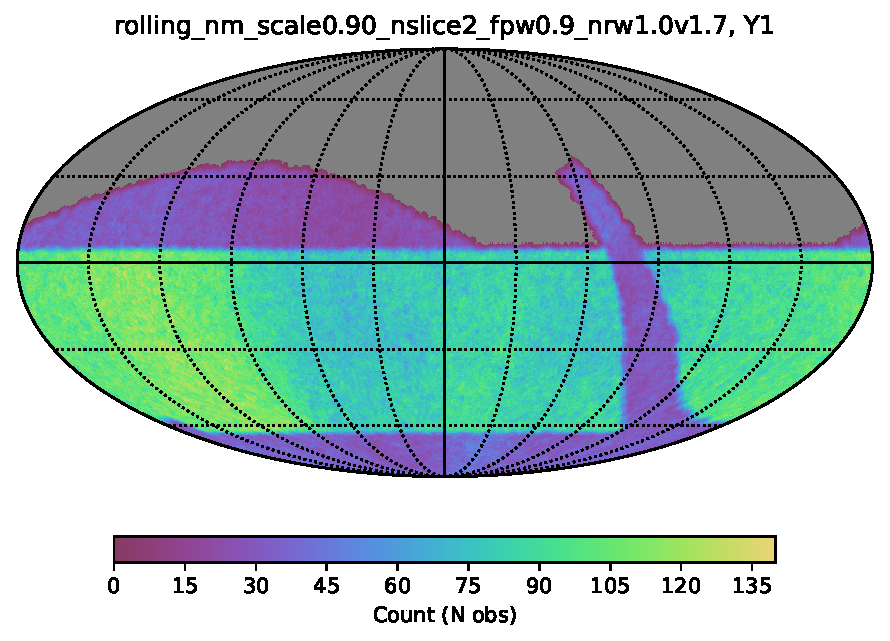
\includegraphics[width=1.75in]{plots/yearly_release/rolling_nm_scale0_90_nslice2_fpw0_9_nrw1_0v1_7_Count_night_lt_365_and_note_not_like_DD_HEAL_SkyMap.pdf}
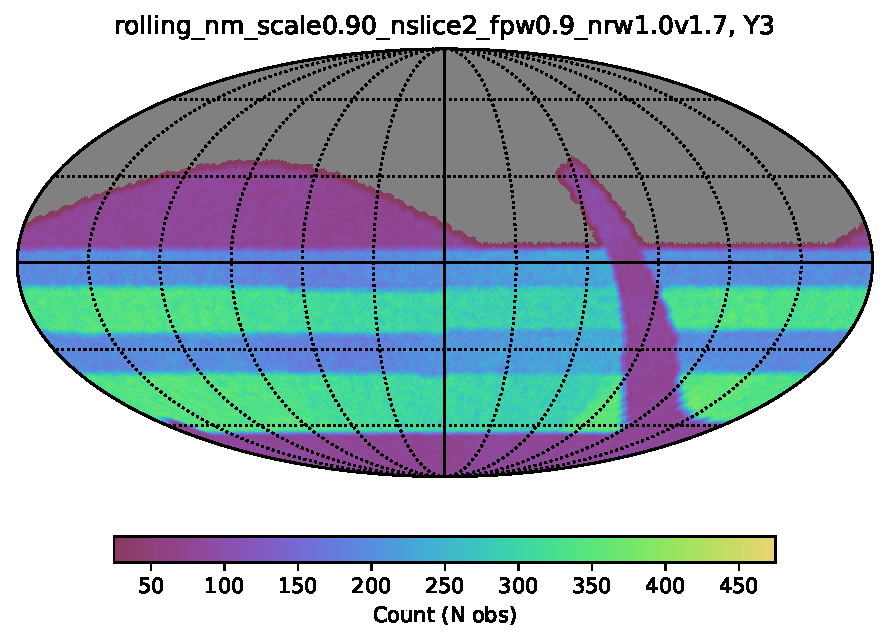
\includegraphics[width=1.75in]{plots/yearly_release/rolling_nm_scale0_90_nslice2_fpw0_9_nrw1_0v1_7_Count_nightlt1095_and_note_not_like_DD_HEAL_SkyMap.pdf}
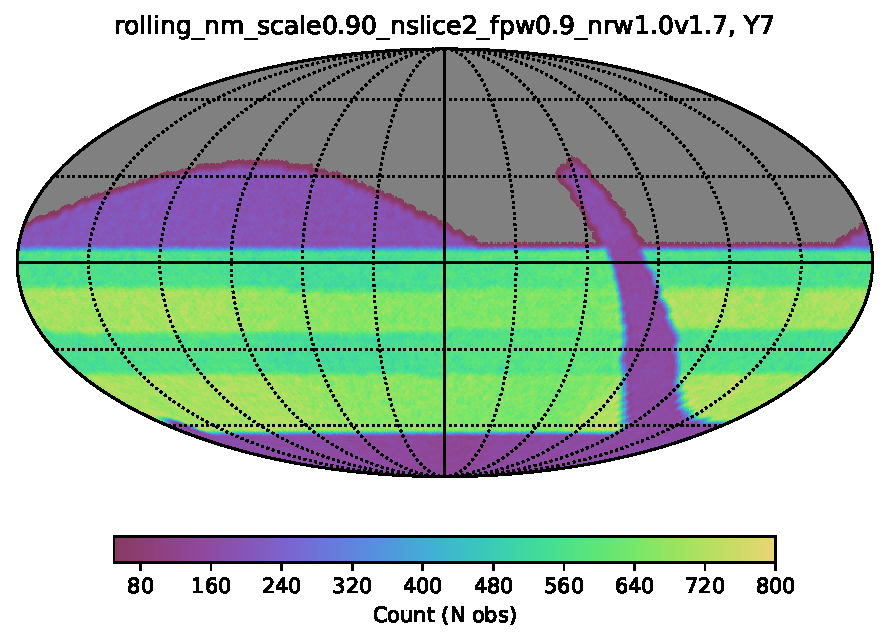
\includegraphics[width=1.75in]{plots/yearly_release/rolling_nm_scale0_90_nslice2_fpw0_9_nrw1_0v1_7_Count_night_lt_2556_and_note_not_like_DD_HEAL_SkyMap.pdf}\\
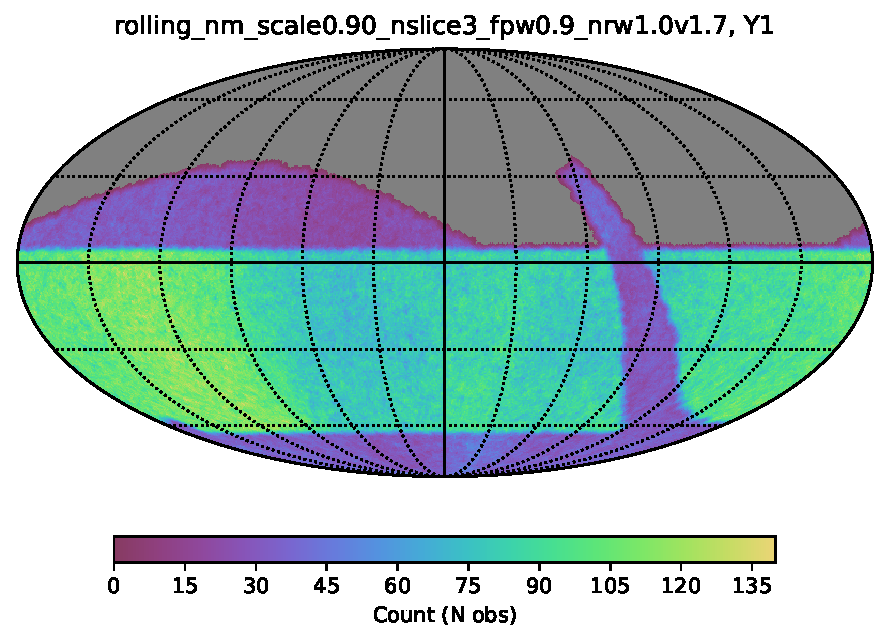
\includegraphics[width=1.75in]{plots/yearly_release/rolling_nm_scale0_90_nslice3_fpw0_9_nrw1_0v1_7_Count_night_lt_365_and_note_not_like_DD_HEAL_SkyMap.pdf}
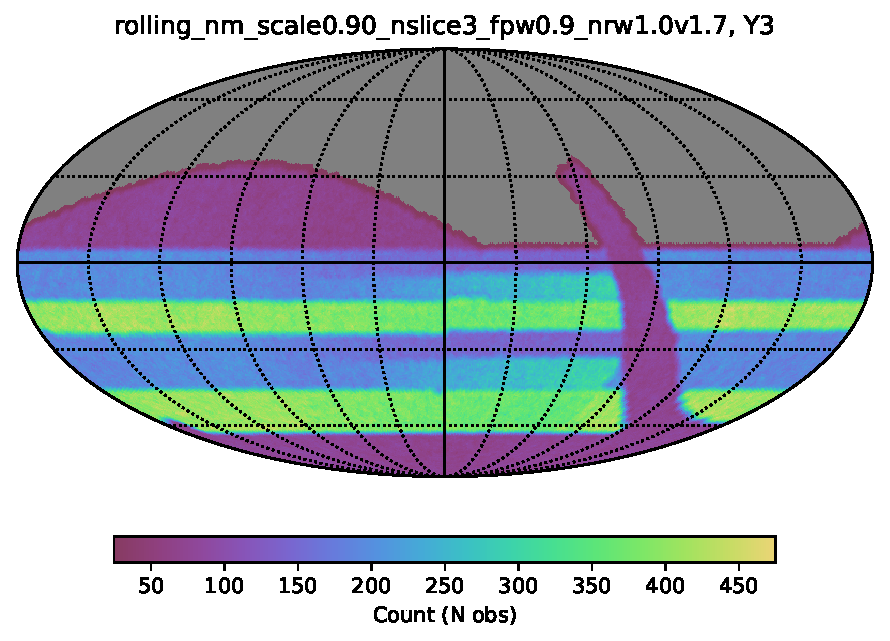
\includegraphics[width=1.75in]{plots/yearly_release/rolling_nm_scale0_90_nslice3_fpw0_9_nrw1_0v1_7_Count_nightlt1095_and_note_not_like_DD_HEAL_SkyMap.pdf}
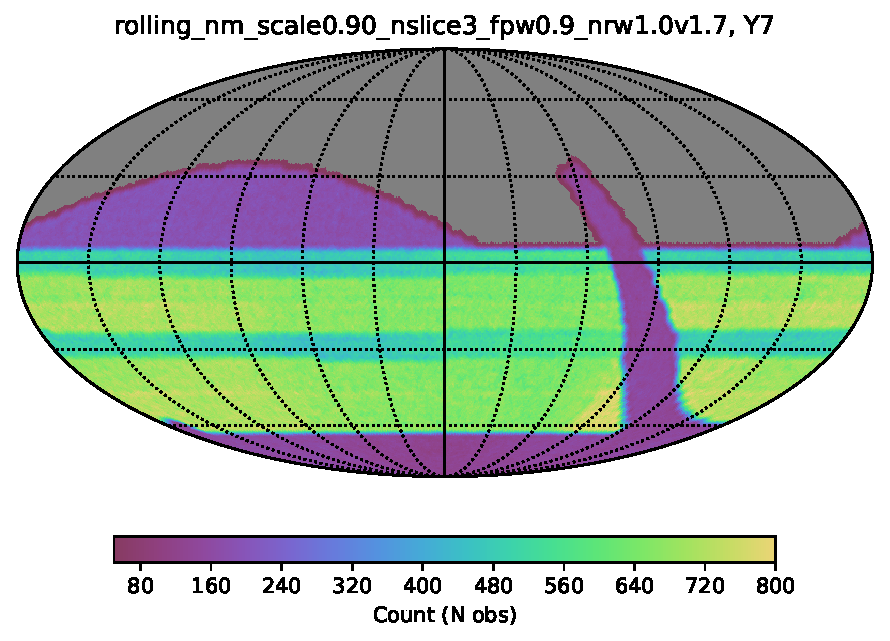
\includegraphics[width=1.75in]{plots/yearly_release/rolling_nm_scale0_90_nslice3_fpw0_9_nrw1_0v1_7_Count_night_lt_2556_and_note_not_like_DD_HEAL_SkyMap.pdf}
\caption{Example of how rolling cadence results in non-uniform coverage for annual data releases. Left shows surveys after 1 year, middle 3 years, right 7 years. Top row show the baseline with no rolling, middle half-sky rolling, bottom third-sky rolling. \label{fig:years}}
\end{figure}

An important consequence of using a rolling cadence is that many annual data releases will not be uniform. Figure~\ref{fig:years} shows how rolling results in uneven coverage of the WFD region after years 3 and 7. This is a consequence of demanding rolling happen for entire observing seasons. The only way to have uniform coverage at data releases with rolling would be to have observing seasons with mixed high and low cadence.



\begin{figure}
\plotone{plots/baseline_nexp2_v1_7_1_10yrs_Hourglass_year_1-2_HOUR_Hourglass.pdf}
\caption{An illustration of which filters are loaded as a function of time in a single year of the survey. All the simulations presented here have a similar behavior with red filters being preferred in bright time. This can result in long gaps in bluer filter coverage even in strongly rolling strategies. Additional gaps are caused by downtime and weather. \label{fig:hour}}
\end{figure}

There are some transient science cases that may still fail to see improvement with our rolling cadences. Figure~\ref{fig:hour} shows how different filters are used depending on the lunar phase. If a transient requires extended coverage in blue filters it may not improve with our current rolling cadence as we still prefer red filters in bright time.

For fast transients ($\sim 1$\ day), rolling may not show much improvement since we are intentionally suppressing taking more than 2 images in a night. However, the 6-band rolling should be useful for fast transient science.

Rolling cadence does not modify the observing season length. Because we use declination bands, the scheduler varies the seasons length across the sky to compensate for under/over subscription. We can potentially extend the observing seasons to better observe long time scale transients, but only by lowering the cadence.



\section{Conclusions}

\begin{itemize}
    \item{We have successfully implemented a variety of rolling cadence strategies on three different survey footprints.}
    \item{Type Ia SNe detection sees a significant improvement with rolling strategies.}
    \item{Fast microlensing events require bulge coverage, and see a decrease in efficiency with the most extreme rolling cadence.}
\end{itemize}


Figure~\ref{fig:classics} shows the final visit distribution for the baseline and rolling cadences are all nearly identical. This implies static science {\emph{at the end of the survey}} should be minimally affected by rolling cadence. During the survey, the WFD will not have even coverage, which will impact static science.

We could expand the half-sky rolling to include and additional rolling cycle (for a total of 4 high cadence and 4 low cadence seasons). It will impact the proper motion precision, but could be a trade off worth exploring. This could also decrease the flexibility to recover from poor weather years near the end of the survey.


% Include all the relevant bib files.
% https://lsst-texmf.lsst.io/lsstdoc.html#bibliographies
\bibliographystyle{aasjournal}
\bibliography{local,lsst,lsst-dm,refs_ads,refs,books}

% Make sure lsst-texmf/bin/generateAcronyms.py is in your path
\section{Acronyms} \label{sec:acronyms}
\input{acronyms.tex}

\end{document}
